\documentclass[conference]{IEEEtran}
\usepackage{times}

% numbers option provides compact numerical references in the text. 
\usepackage[numbers]{natbib}
\usepackage{multicol}
\usepackage[bookmarks=true]{hyperref}

\pdfinfo{
   /Author (author)
   /Title  (title)
   /CreationDate (D:20101201120000)
   /Subject (Robots)
   /Keywords (Robots)
}

\usepackage{microtype}
\usepackage{amsmath,amssymb}
\usepackage{paralist}
\usepackage{mdframed}
\usepackage{xcolor}
\usepackage{tikz}
\usepackage{amsthm}
\usepackage{amssymb}
\usepackage{amsthm}
\usepackage{colonequals}
\newtheorem{theorem}{Theorem}
\theoremstyle{remark}
\newtheorem{remark}{Remark}
\newtheorem{example}{Example}

\usetikzlibrary{patterns,arrows,backgrounds,calc,shapes,shadows,decorations.pathmorphing,decorations.pathreplacing,automata,shapes.multipart,positioning,shapes.geometric,fit,circuits,trees,shapes.gates.logic.US,fit,decorations.markings}

\tikzset{sstate/.style={circle, draw=black, inner sep=1pt}}

\makeatletter
\let\MYcaption\@makecaption
\makeatother

\usepackage[font=footnotesize]{subcaption}

\makeatletter
\let\@makecaption\MYcaption
\makeatother

\newcommand{\NN}{\mathbb{N}}
\newcommand{\mc}{\mathcal{D}}
\newcommand{\sg}{\mathcal{G}}
\renewcommand{\path}{\xi}
\newcommand{\eventually}[1]{\lozenge^{\leq #1}}
\newcommand{\sched}{\sigma}
\newcommand{\Sched}{\Sigma}
\newcommand{\pol}{\sched}
\newcommand{\Distr}{\ensuremath{\textsl{Distr}}}
\newcommand{\act}{\alpha}
\newcommand{\Act}{A}
\newcommand{\scthreshold}{p}
\newcommand{\target}{s_{\top}} 
\newcommand{\sink}{s_{\bot}}
\newcommand{\randomness}{h}
\newcommand{\last}[1]{{#1}_\downarrow}
\newcommand{\pOneSched}{\mathbf{ego}}
\newcommand{\POneScheds}{\Sigma_\pOne}
\newcommand{\PTwoScheds}{\Sigma_\pTwo}
\newcommand{\pTwoSched}{\mathbf{env}}
\newcommand{\pOne}{\mathsf{ego}}
\newcommand{\pTwo}{\mathsf{env}}
\newcommand{\horizon}{\tau}
\newcommand{\solutions}{\mathbb{S}}

\newcommand{\pathslbl}{\Xi}
\newcommand{\Paths}[2][]{\pathslbl^{#2}_{#1}}
\newcommand{\POnePaths}[2][]{{\pathslbl^{#2}_{#1}}/_{\downarrow_{1}}}
\newcommand{\PTwoPaths}[2][]{{\pathslbl^{#2}_{#1}}/_{\downarrow_{2}}}
\newcommand{\PiPaths}[2][]{{\pathslbl^{#2}_{#1}}/_{\downarrow_{i}}}
\newcommand{\unrolled}[2]{\textsf{Tree}(#1,#2)}
\newcommand{\induced}[2]{#1[#2]}
\newcommand{\causalprob}[2]{\Pr(#1\mid\mid#2)}
\newcommand{\expOver}[2]{\mathbb{E}_{#1}[#2]}



\setlength\marginparwidth{110pt}
\newcommand{\colorpar}[3]{\colorbox{#1}{\parbox{#2}{#3}}}
\newcommand{\marginremark}[3]{\marginpar{\colorpar{#2}{\linewidth}{\color{#1}#3}}}
\newcommand{\commentside}[2]{\marginpar{\color{#1}\tiny#2}}
\newcommand{\TODO}[1]{\commentside{teal}{\textsc{Todo:} #1}}
\newcommand{\REMARK}[1]{\commentside{teal}{\textsc{Remark:} #1}}\newcommand{\sj}[1]{\marginremark{black}{red!10!white}{\scriptsize{[SJ]~ #1}}}
\newcommand{\mvc}[1]{\marginremark{black}{gray!10!white}{\scriptsize{[MVC]~ #1}}}


%\institute{University of California, Berkeley, CA, USA}


\begin{document}

% paper title
\title{Entropy-Guided Control Improvisation}

% You will get a Paper-ID when submitting a pdf file to the conference system
\author{Author Names Omitted for Anonymous Review. Paper-ID [add your ID here]}

%\author{\authorblockN{Michael Shell}
%\authorblockA{School of Electrical and\\Computer Engineering\\
%Georgia Institute of Technology\\
%Atlanta, Georgia 30332--0250\\
%Email: mshell@ece.gatech.edu}
%\and
%\authorblockN{Homer Simpson}
%\authorblockA{Twentieth Century Fox\\
%Springfield, USA\\
%Email: homer@thesimpsons.com}
%\and
%\authorblockN{James Kirk\\ and Montgomery Scott}
%\authorblockA{Starfleet Academy\\
%San Francisco, California 96678-2391\\
%Telephone: (800) 555--1212\\
%Fax: (888) 555--1212}}


% avoiding spaces at the end of the author lines is not a problem with
% conference papers because we don't use \thanks or \IEEEmembership


% for over three affiliations, or if they all won't fit within the width
% of the page, use this alternative format:
% 
%\author{\authorblockN{Michael Shell\authorrefmark{1},
%Homer Simpson\authorrefmark{2},
%James Kirk\authorrefmark{3}, 
%Montgomery Scott\authorrefmark{3} and
%Eldon Tyrell\authorrefmark{4}}
%\authorblockA{\authorrefmark{1}School of Electrical and Computer Engineering\\
%Georgia Institute of Technology,
%Atlanta, Georgia 30332--0250\\ Email: mshell@ece.gatech.edu}
%\authorblockA{\authorrefmark{2}Twentieth Century Fox, Springfield, USA\\
%Email: homer@thesimpsons.com}
%\authorblockA{\authorrefmark{3}Starfleet Academy, San Francisco, California 96678-2391\\
%Telephone: (800) 555--1212, Fax: (888) 555--1212}
%\authorblockA{\authorrefmark{4}Tyrell Inc., 123 Replicant Street, Los Angeles, California 90210--4321}}


\maketitle

\begin{abstract}
Declarative constraints are a powerful tool to define high-level controllers. 
However, most algorithms that synthesise controllers from these constraints construct deterministic policies -- which limits robustness and unpredictability.  
Control improvisation aims to overcome these weaknesses. Key are three types of constraints: Hard constraints describe behavior that must occur, 
soft constraints describe behavior that typically occurs, and a randomization constraint ensures variance in the behavior. 
We provide the first control improvisation framework, based on causal entropy to describe randomization, that supports to adverserial and probabilistic environments. These features allow us to synthesise powerful robust policies that generatate unpredictable behavior. 

\end{abstract}

\IEEEpeerreviewmaketitle

%\maketitle\sj{Daniel?}
%\begin{abstract}
%	Efficacious controller synthesis is a key ingredient in the design and analysis of complex systems. We study the design of controllers that have a high entropy, that is, whose behavior or nature is surprising. The synthesis of such controllers is key in domains like testing and security. 
%	In particular, our paper studies control improvisation and compares them with randomly sampling adequate policies. The only difference in obtained policies is in their notion of entropy, but the problems are significantly different.  We illustrate and contrast their merits and limitations. Furthermore, we provide algorithms that solve both control improvisation problems. Prominently, we solve the control improvisation problem for Markov decision processes by relating it to recent results from inference from demonstrations, and then extend this approach to stochastic games. We present a prototypical implementation that efficiently solves controller synthesis problems from the security and testing domain. 
%\end{abstract}
\section{Introduction}
% Declarative Constraints ar neat idea.
The use of declarative specifications, e.g. in the form of temporal logic formulas, has become a popular way to construct high-level robot controllers~\cite{DBLP:conf/iros/HorowitzWM14, DBLP:conf/rss/WongEK14, DBLP:conf/iros/HeLKV17, DBLP:conf/icra/FuATP16, DBLP:conf/icra/HeWKV19, DBLP:journals/arobots/MoarrefK20, DBLP:conf/icra/KantarosM0P20}.
% Synthesis closes the gap.
Given a user provided specification, \emph{synthesis} algorithms aim
to automatically create a control policy that ensures that the
specification is met, or explain why such a policy does not
exist. Together, synthesis and declarative specifications facilitate
quickly and intuitively solving a wide variety of control tasks.  For
example, consider a delivery drone operating in a workspace. One may
specify the drone should ``within 10 minutes, visit four locations (in any
order) \emph{and} avoid crashing.''. A synthesis tool may then create a
finite state controller which guarantees this specification is met,
under a particular world model.
% Declarative Synthesis need not produce variety.  
Importantly, while there may be many controllers that conform to the
provided specification, many synthesis algorithms provide a
single, often deterministic, policy.  For instance, in our drone
example, a synthesized controller may generate only a single path
through the workspace.

% On the importance of being varied.
In some settings, such policies however are undesirable.  First, in
many tasks, the predictability (or bias) of the policy may be a
liability.  Example include
patrolling~\cite{DBLP:journals/ior/AlpernMP11}, behavior prediction
and inference~\cite{DBLP:conf/cav/Vazquez-Chanlatte20}, and creating
controller harnesses for fuzz testing (see motivating
example). Second, synthesis algorithms work on \emph{idealized}
models, and thus any policy that over commits to any given model quirk
may in practice yield poor performance. In such settings,
randomization is known to make policies more robust against worst-case
deviations~\cite{mceThesis, maxEntAnswer}. Unfortunately, traditional
synthesis problems result policies that need not (and typically do
not) exhibit randomization.

% Propose CI and highlight new features.
To address these potential deficits, we advocate for the adoption of
the recently proposed control
improvisation~\cite{DBLP:conf/cav/FremontS18,DBLP:conf/fsttcs/FremontDSW15}
framework, in which one specifies a controller with three types of
declarative constraints. (1) \emph{Hard constraints} that, as in the
classical setting, must be satisfied, (2) \emph{soft constraints} that
on most executions should hold, and (3) \emph{randomization
constraints} that ensure that a synthesized policy does not overly
commit to a particular action or behavior. 
The key challenge is that randomization and performance in the form of soft constraints form a natural trade off.

Unfortunately, control
improvisation has so far been limited to deterministic domains where
uncertainty is resolved adversarially. This assumption is often too
restrictive and leads (together with the soft/hard constraints) to
conservative policies or common situations in which the synthesis
algorithm cannot be employed at all. To overcome this weakness, we
develop a theory of control improvisation in stochastic games which
admit arbitrary \emph{combinations} of adversarial and probabilistic
uncertainty, including unknown or imprecise transition
probabilities. as the policy is no longer the only
source of randomization, this extension requires a different
view on randomization constraints.

Technically, we formulate our problem on \emph{simple stochastic
games}~\cite{DBLP:conf/dimacs/Condon90}, an extension of Markov decision processes that divides states
between controllable states and uncontrollable (or adversarially
controlled) states. \emph{Soft constraints} are finite horizon
temporal properties with a threshold on the worst-case probability of
that the property holding by the end of the episode. \emph{Hard
constraints} are soft constraints satisfied with probability 1. In
contrast to other work on control improvisation, we adopt the notion
of causal entropy as natural means to formalize \emph{randomness
constraints}.  Causal entropy is a prominent notion in directed
information theory \sj{Add citation?} that strongly correlates with robustness in the
(inverse) reinforcement learning setting~\cite{mceThesis,
maxEntAnswer}. We refer to this variant of control improvisation as
Entropic Reactive Control Improvisation (ERCI) and show that ERCI
conservatively extends reactive control improvisation~\cite{DBLP:conf/cav/FremontS18} to stochastic
games. More precisely, while we focus on stochastic games, entropy can
be used in the non-stochastic setting and yields results analogous to
the reactive control improvisation. ERCI also conservatively extends  classical policy synthesis in stochastic games, i.e. synthesis in absence of randomness constraints as, e.g., implemented in PRISM-games~\cite{DBLP:journals/sttt/KwiatkowskaPW18}.


%We argue that soft constraints can naturally be considered as an
%optimization objective which one can trade-off for more randomization.
%Indeed, our method strongly relies on the computation of a
%Pareto-front that explores the trade-off between randomization and
%optimizing the soft constraint using the notion of rationality. This
%means that rather than asking the user to fix rather arbitrary
%threshold values for both types of constraints, we may visualize the
%trade-off between these two entities.
%
\mypara{Contributions}
In summary, this paper contributes ERCI, an algorithmic way to trade 
performance and randomization in stochastic games. As we motivate in the example below, the support for stochastic games that combine both
adversarial and probabilistic behavior in an environment allows for
modeling flexibility, admitting applicability to new domains. To
support this extension, the paper proposes and shows the benefits
formulating randomization constraints with causal entropy.  Finally,
this paper contributes the necessary machinery as well as a
prototypical implementation.

\mypara{Overview} This paper is structured as follows. We begin
with a motivating example (Sec.~\ref{sec:motivating}). Then we
provide preliminaries and formalize the ERCI problem statement in
Sec.~\ref{sec:problem}. Next, in Sec.~\ref{sec:convex}, we cast ERCI
as a multi-objective optimization problem and study properties of the
solution set. With this technical machinery developed,
Sec.~\ref{sec:mdps} re-frames existing literature on maximum causal
entropy inference and control to derive an algorithm for Markov
Decision Processes.  Then in Sec.~\ref{sec:sgs}, we provide an
algorithm for the general case of stochastic games. Finally, we
conclude with an empirical evaluation (Sec.~\ref{sec:empirical}) and a
comparison with other control improvisation formulations and other
related work (in Sec.~\ref{sec:related}).



%%% Local Variables:
%%% mode: latex
%%% TeX-master: "main"
%%% End:

\section{Motivating Example}

\begin{figure}
  \centering
  \scalebox{0.4}{
    \import{imgs/}{motivating_example.pdf_tex}
    }
\caption{Plans for different battery models}	
\end{figure}

\begin{figure*}

\caption{Plans for different models of drone $E$}	
\end{figure*}


We consider high-level planning for drones. We consider a setting with a controllable drone $D$ and in presence of a secondary drone $E$. 
We partition the airspace into different zones. Four zones are marked as special points of interest (POIs).
One of the zones in a corner is a recharge station, where $D$ initially starts. $E$ starts in the opposite corner. We assume perfect observability.  
For safety, our plan must (\emph{hard constraint}) ensure that the two drones are never in the same zone. We are only interested in plans that visit the four POIs within a given time horizon (\emph{hard constraint}).
We should (\emph{soft constraint}) ensure that we do not run out of battery with high probability. 
Our aim is to create a plan such that the paths of $D$ within its environment are maximally unpredictable (random constraint), i.e., we want to maximally randomize over the paths that satisfy the constraints. Due to the nature of the soft constraint, some of the paths that we include may violate this constraint.  We apply our novel entropy-guided control improvisation. In the folllowing, we discuss different aspects of this setting.

Let us first start in absence of $E$. 
The main task here is to ensure power-aware scheduling, i.e., depending on the state of charge of the battery, we want to adapt our plan. Crucial in this is an adequate model of the battery. 
Both the battery quality itself and the power consumption are, however, uncertain. 
In particular, we may model that in every step deterministically the average power is consumed, but this plan will not be robust to any other behavior, and the plan is unrealistic~\cite{DBLP:conf/cyphy/HermannsKN15}. Typically, in synthesis, the other extreme is assumed (any amount of power can be drawn in every step). In this setting, this assumption leads the battery to be discharged with the maximal power consumption -- while this is clearly too pessimistic -- there is no policy that satisfies our constraints.
We use a model in which we discretize the battery charge, and in every time step the battery charge decrements by one step with some probability $p$. 
Overall, this yields a binomial distribution over the maximal steps until the battery is depleted.
In Fig.~\ref{fig:motivating:batteries}, we show paths with a larger and smaller battery. As to be expected, the larger battery allows for more freedom in randomizing, as it is easier to meet the soft constraint.


Orthogonally, let us consider drone $E$. 
In the best case, drone $E$ is a delivery drone delivering packages along a fixed route. We can encode this route into the model. 
Compare Fig.~\ref{} without a drone $E$ and Fig.~\ref{} with drone $E$ flying the path marked in red. 
We can see how fewer paths meet the hard constraint, and thus, $D$ randomizes over fewer paths. 
The plans in Fig.~\ref{} are not very robust: what if $E$ occasionally decided to return to its base (e.g., to recharge). More precisely, in Fig.~\ref{} we illustrate the policy for $D$ if we assume that $E$ flips a biased coin in every step in which it decided to turn around.
We observe that this decreases the paths that satisfy the hard guarantee (not crashing) and indirectly also means that it becomes more likely that we deplete the battery due to evading $E$.
Finally, rather than assuming some stochastic behavior where $E$ turns around, we may want to not make any assumption on under which circumstances or what probability $E$ turns. 
The difference is more subtle: changing from randomization to adversarial behavior of $E$ does not change the set of paths that violate the hard constraint, $D$ will need to evade $E$ more often, yielding higher battery consumption. 
More generally, the difference between assuming random behavior of $E$ and adversarial behavior is as follows: In the latter case, we are interested in a policy that is good for any behavior of $E$, that is, it is good in the worst-case, whereas assuming (uniform) random behavior for $E$ in expectation, but does not give guarantees on the worst-case. Generally, optimizing for the worst-case is overly pessimistic.

A natural criticism for stochastic models is the dependence on fixed probabilities.
 In our example, we may have observed $E$'s behavior and extracted (point-)estimate probabilities $p$ using inverse reinforcement learning. In absence of (enough or reliable) data, we can combine adversarial choices and stochastic behavior such that we may model ranges of possible transition probabilities. 
 More precisely, we support interval-valued transition probabilities. Consider the delivery-drone $E$. Rather than inferring a point-estimate from data, we may have inferred that the probability of turning around is in the interval $[p - \varepsilon, p + \varepsilon]$ for adequate values of $p$ and $\varepsilon$.  Furthermore the actual probability may even depend on aspects of the current state. 

The strength of the (entropy-guided) control improvisation framework is that we can combine all these aspects into a single computational model, which is very flexible. For example, we use an interval-based model for the turn-around probability and a battery model to create the plans visualised in Fig.~\ref{}.
Finally, one aspect we want to highlight here is the implicit construction of a Pareto-curve that shows how randomization and performance yield a tradeoff. This means that rather than a-priori selecting threshold for entropy and the probability of not running out of battery, we obtain a variety op options and select the trade-off that is most satisfactory. Consider Fig.~\ref{}.



%%% Local Variables:
%%% mode: latex
%%% TeX-master: "main"
%%% End:

\section{Problem Statement}
This section formalizes the problem statement. We show that our problem statement is a conservative extension of the existing reactive control improvisation framework and we reformulate our problem statement in terms of finding a Pareto-curve. We start with some necessary definitions and notations.


\subsection{Stochastic Games}
An (alternating, 2.5-player) \emph{stochastic game} (SG) is a tuple $\sg = \langle S, \iota, \Act, P \rangle$. A finite state $S = S_1 \cup S_2 \cup S_E$ is partitioned into a set $S_1$ of player-1 states, a set $S_2$ of player-2 states, and a set $S_E$ of environment states. $\iota \in S_1$ is the initial state, $\Act = \Act_1 \cup \Act_2$ is a finite set of actions, and $P\colon S \times \Act \rightarrow \Distr(S)$ is defined by a set of three transition functions: $P_1\colon S_1 \times \Act_1 \rightarrow S_2$, $P_2\colon S_2 \times \Act_2 \rightarrow S_E$, $P_E\colon S_E \rightarrow \Distr(S_1)$.
If $\Act_2$ is a singleton set, then $\sg$ is an \emph{Markov decision process}.
If both $\Act_1$ and $\Act_2$ are singleton sets, then $\sg$ is a \emph{Markov chain}. If $P_E(s)$ is a Dirac distribution for every $s \in S_E$, then, $\sg$ is called \emph{deterministic}.

In this paper, it is helpful to consider $P_E$ as being defined using an auxiliary notion of environment actions $\Act_E$, a deterministic environment transition relation $P_{\hat{E}}\colon S_E \times A_E \rightarrow S_1$ and (memoryless, randomized) environment-scheduler $S_E \rightarrow \Distr(A_E)$.
\sj{I want to put this text where we use this for the first time.}

A finite path $\pi = s_0 \xrightarrow{a} s_1 \xrightarrow s_2$

\paragraph{Policies.} 
As standard, before we can define probabilities, all nondeterminism needs to be resolved. We do this with the notion of a policy. 

\sj{add unrolling}


\paragraph{Properties.}
We consider finite horizon reachability properties.

\paragraph{Entropy}


Define entropy on a random variable.\sj{Do}

Define entropy on a Markov chain\sj{Do}



\subsection{Control Improvisation and random policies}

\begin{mdframed}
Given a SG $\sg$ with target-states $T$ and $G$ and a horizon $h$, does there exists a policy $\sched_1 \in \Sched_1$  such that for every policy $\sched_2 \in \Sched_2$ and with $\sched = \langle \sched_1, \sched_2 \rangle$ it holds that 
\begin{compactenum}
	\item $\Pr^\sg_{\sched}(\eventually{h} T) \geq 1$
	\item $\Pr^\sg_{\sched}(\eventually{h} G) \geq \lambda$
	\item $H(\sg[\sched]) \geq \kappa$
\end{compactenum}
\end{mdframed}
Rather than fixing $\kappa$ a priori, we are often interested in limiting the \emph{regret}: The last point then becomes:
$H(\sg[\sched]) \geq (1-\delta) \cdot H(\sg[\sched^{*}])$, where $\sched^{*}$ .... \sj{I am not sure how to define this concisely.} 


Before we continue, we want to establish that Control improvisation problem is a conservative extension of deterministic case as investigated in~\cite{}.
\begin{lemma}
	
\end{lemma}


\begin{mdframed}

\begin{compactenum}
	\item $\Pr^\sg_{\langle \sched_1,\sched_2 \rangle}(\eventually{h} T) \geq 1$
	\item $\Pr^\sg_{\langle \sched_1,\sched_2 \rangle}(\eventually{h} G) \geq \lambda$ 
\end{compactenum}
\end{mdframed}
\sj{Define randomly selected policy}







\section{The Control Improvisation Problem for MDPs}
\color{black!50}
We consider $P$ as being defined using an auxiliary notion of environment actions $\Act_E$, a deterministic environment transition relation $P_{\hat{i}}\colon S_i \times \Act_i \rightarrow A_E$ and a (memoryless, randomized) environment-scheduler $A_E \rightarrow \Distr(S)$.



It is convenient to talk about a third player, $\mathsf{rnd}$, that owns all states with $|\Act|$\sj{needs available actions}
\color{black}

We present an algorithm for the control improvisation problem for MDPs. The key insight is to reuse ideas from policy inference from specifications~\cite{DBLP:conf/cav/Vazquez-Chanlatte20}.
In the next section, we extend this idea to SGs. 

\begin{figure}
\begin{subfigure}{0.3\columnwidth}
\centering
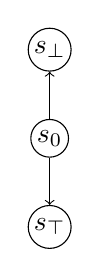
\begin{tikzpicture}	
	\node[sstate] (si) {$s_0$};
	\node[sstate,above=0.6cm of si] (s0) {$\sink$};
	\node[sstate,below=0.6cm of si] (s1) {$\target$};
	\draw[->] (si) -- (s0);
	\draw[->] (si) -- (s1);
	
\end{tikzpicture}
\caption{}
\end{subfigure}
\begin{subfigure}{0.3\columnwidth}
\begin{tikzpicture}	
\end{tikzpicture}
\caption{}
\end{subfigure}
\begin{subfigure}{0.3\columnwidth}
\begin{tikzpicture}	
\end{tikzpicture}
\caption{}
\end{subfigure}


\end{figure}



\subsection{Soft constraint vs randomness}
\paragraph{Max randomness without soft constraint}
The uniform random policy maximises randomness.
\begin{remark}
Notice that here, it is important that our induced Markov chain contains the state choices as well.	
\end{remark}


\paragraph{Monotonicity}
\sj{add lemma}
We can (conceptually) sort all policies by their induced reachability to reach states $G$, i.e., by the (quantitative) satisfaction of the soft constraint. For each policy, we can plot the associated maximal entropy, $H^*(\lambda) = \sup_{\sched} \{ H(\sg[\sched]) \mid \Pr_{\sched}(\eventually{h} G) = \lambda\}$, see Fig.~\ref{fig:entropyvspsat}.
The policy that maximises the entropy is (typically) somewhere in the middle--and the function is monotonically decreasing on both sides. 
In this paper, we are only interested in the right side of the graph:
We first construct the max-entropy policy $\sched^*$. If the induced probability $\Pr_{\sched^*}(\eventually{h} G) \geq \lambda$ and the associated entropy $H(\sg[\sched^*]) \geq \kappa$, then we found a solution to the CI problem. If $\Pr_{\sched^*}(\eventually{h} G) \geq \lambda$ but $H(\sg[\sched^*]) \geq \kappa$, then the CI problem is unsatisfiable (recall that $\sched^*$ maximizes entropy).
The remaining case is that $\lambda \geq \Pr_{\sched^*}(\eventually{h} G)$, i.e., the right side of the graph.
For that, it holds that the higher $\lambda$, the lower $\sup_{\sched} \{ H(\sg[\sched]) \mid \Pr_{\sched}(\eventually{h} G) = \lambda\}$~\sj{Can we cite something, do we need to prove this ourselves?}. 
\begin{figure}
\begin{tikzpicture}[scale=3]
	 \draw[->] (-0.05, 0) -- (1, 0) node[right]{$\Pr_\sched(\eventually{h}G)$};
  	\draw[->] (0, -0.05) -- (0, 0.8) node[above] {$H^*$};
  	\draw[-,dashed] (0.4,0) -- (0.4,0.5184);
  	\draw[-,dashed] (0.0,0.5184) -- (0.4,0.5184);
  \draw[ domain=0:1, smooth, variable=\x, blue] plot ({\x}, {15*(1-\x)*(1-\x)*(1-\x)*\x*\x});
\end{tikzpicture}	
\caption{Entropy vs reachability probability for the soft constraint}
\label{fig:entropyvspsat}
\end{figure}
Result: A computation tree, computing the max entropy over schedulers that achieve the goal with prob exactly $\lambda$.
A variant in which we explore the trade-off between soft constraint and entropy is a simple extension that employs a binary search.
\subsection{Entropy maximization for a fixed reachability probability}

An optimal policy follows the Bellman equation
\[ V(s,h)  = \max_{\act \in \Act} \sum_{s'} P(s,\act,s') \cdot V(s',h-1),\]
where $V$ denotes the value, which here corresponds to the $h$-step reachability probability from state $s$ onwards.
In particular, in every step, we take the actions that maximize the probability to reach the target (within the horizon). 
If we now want to reduce the probability to reach the goal (and thereby allow to increase the entropy) we can select in every step (with some probability) one or more of the suboptimal actions. We call this possibility \emph{wiggle room}. 
\paragraph{How to wiggle?}
We should pick suboptimal actions in such a way that we maximize the overall entropy. Let us therefore generalize the Bellman equation:

We observe that for $\theta \rightarrow \infty$, this equation matches the (traditional) Bellman equation. 
Furthermore, for $\theta \rightarrow 0$, this equation yields a policy that maximises entropy.
Thus, intuitively, we can span the whole (right part of) the graph as depicted in Fig.~\ref{fig:entropyvspsat}.

\sj{Here we need to add some more formal argument}

\paragraph{An Algorithm for control improvisation}

We use binary search (more precisely: root finding of a monotonic function) to select a 

The algorithm 

\sj{Do we know the complexity of the decision problem? To encode it in a set of constraints we need extended polynomial equations (with exponents, that is), right?}



 

\section{The Control Improvisation Problem for SGs}
\paragraph{Maximising entropy against an adverserial player}

\subsection{Playing against deterministic adverseries}
To formalise our argument
\paragraph{Reformulation as a set of MDPs}

\paragraph{}


\subsection{Randomizing adversaries will not play better}

\subsection{Non-observable adversaries}

\section{Control improvisation versus Policy Sampling}
In this section, we discuss the nature of the randomness as imposed by the CI problem, and relate this to improvising policies, i.e., to randomly sampling policies that satisfy the hard and soft constraint.


Before we continue, we want to establish that Control improvisation problem is a conservative extension of deterministic case as investigated in~\cite{}.
\begin{mdframed}
\textbf{The Deterministic (Reactive) Control Improvisation (DCI) Problem~\cite{}}:
Given a \emph{deterministic} SG $\sg$, finite path sets $X_\psi$ and $X_\varphi$, and a threshold $p \in (0,1)$,  find a $\pOne$-policy $\pOneSched \in \POneScheds$  such that for every $\pTwo$-policy $\pTwoSched \in \PTwoScheds$ 
\begin{compactenum}
\item (\emph{hard constraint}) $\Pr^\sg_{\sched}(X_\psi) \geq 1$
	\item (\emph{soft constraint)} $\Pr^\sg_{\sched}(X_\varphi) \geq \scthreshold$
	\item (\emph{randomness constraint}) $\Pr(\path) \leq \delta \text{ for all } \path \in \Paths[h]{\sg[\sched]}$.
\end{compactenum}
\end{mdframed}

\begin{theorem}
	For deterministic SGs, the ERCI and DCI problem coincide.
\end{theorem}
We defer a discussion and a precise statement to Lemma~\ref{}.

%\begin{mdframed}
%
%\begin{compactenum}
%	\item $\Pr^\sg_{\langle \sched_1,\sched_2 \rangle}(\eventually{h} T) \geq 1$
%	\item $\Pr^\sg_{\langle \sched_1,\sched_2 \rangle}(\eventually{h} G) \geq \lambda$ 
%\end{compactenum}
%\end{mdframed}
%\sj{Define randomly selected policy}
%\sj{Describe in terms of pMDPp}

\section{Discussion}


\section{Implementation and Empirical Evaluation}

\section{Related work}
\color{red}
\cite{DBLP:journals/corr/abs-2009-10883}
\cite{DBLP:journals/jcss/BrazdilCFK17}
\color{black}



Path-finding has long been considered a multi-objective problem itself~\cite{DBLP:conf/icra/AmigoniG05,DBLP:journals/eswa/NazarahariKD19,DBLP:conf/icml/XuTMRSM20}.
These works differ prominently in two aspects: they do not trade-off randomization and performance, and they do not trade-off declarative and formal constraints with the accompanying formal guarentees, but are more search-based. 
Finding policies that optimize reward objectives is well-studied in the field of reinforcement learning, and has been extended to generate Pareto-fronts for multiple objectives~\cite{DBLP:conf/icml/NatarajanT05,DBLP:conf/adprl/ParisiPSBR14}.

Synthesis in MDPs with multiple hard and soft constraints (often over indefinite horizons) is a well-studied problem~\cite{DBLP:conf/stacs/ChatterjeeMH06,DBLP:conf/tacas/EtessamiKVY07,DBLP:conf/atva/ForejtKP12,DBLP:journals/fmsd/RandourRS17}.  In this setting, one generates deterministic policies and their convex combinations. Put differently, randomization is \emph{not an objective}, but rather a consequence. Interestingly, in \cite{DBLP:conf/tacas/DelgrangeKQR20} one even argues for the \emph{absence} of randomization in various domains.  
The original results sparked interest in different extension to MDPs and the type of soft constraints, such as continuous MDPs \cite{DBLP:journals/csysl/HaesaertNS21} and continuous-time MDPs~\cite{DBLP:conf/cav/QuatmannJK17},  cost-bounded reachability \cite{DBLP:journals/jar/HartmannsJKQ20}, or mean-payoff properties~\cite{DBLP:journals/corr/abs-1104-3489}. 
The algorithms have also been extended towards stochastic games~\cite{DBLP:conf/mfcs/ChenFKSW13,DBLP:journals/sttt/KwiatkowskaPW18}.
Finally, notions of lexicographic multi-objective synthesis~\cite{DBLP:conf/cav/ChatterjeeKWW20} -- in which one optimizes a secondary criterion among all policies that are optimal with respect to a first criterion bare some resemblance with the algorithm we consider. 
These algorithms have been put in a robotics context in~\cite{DBLP:journals/ijrr/LacerdaFPH19}.


\bibliographystyle{plainnat}
\bibliography{bibliography}

\end{document}
